% \tm{Just noting the title. In the Slack, you proposed `planning with belief using justified perspectives', which I think captures the work better}
% \gh{Sure. But what should the acronyms be? PBJP or PWBUJP, or PWBJP?}
\section{Introduction and Motivation}
\label{sec:intro}
In epistemic planning problems, agents need to reason about the ontic world and the epistemic world. 
There is extensive research on epistemic logic reasoning and epistemic planning, each with its own strengths and limitations. 
%The \emph{Dynamic Epistemic Logic} (DEL) ~\cite{DBLP:journals/jancl/BolanderA11,DBLP:conf/ecsi/Bolander14} based approach uses an event model to update an agent's belief through observations over actions.
%This approach uses different actions to update the ontic state, the epistemic state, and the agent's observability.
%There are two main drawbacks with DEL: 1)
%it has to explicitly model the high-order observability between agents; 
%2) it requires the modeller to understand the domain and the effects of each action with respect to the ontic an epistemic worlds.
Most epistemic planning approaches either explicitly maintain all epistemic relations, such as Kripke frames \cite{DBLP:conf/aips/KominisG15,DBLP:journals/jancl/BolanderA11,DBLP:conf/ecsi/Bolander14}, or require an expensive pre-compilation step to convert an epistemic planning problem into a classical planning problem~\cite{DBLP:journals/ai/MuiseBFMMPS22}, which grows exponentially w.r.t. the depth of the epistemic formula used.

Recently, \citet{Hu2022-ul} proposed a lazy-evaluation approach to epistemic planning called Planning with Perspectives (PWP).
They use Functional STRIPS (F-STRIPS) \cite{geffner2000functional} to separate epistemic reasoning from planning by modelling an agent's perspective using external functions, which can be customised for particular domains. 
The agent perspective function defines which variables each agent `sees' in each state, and from this, a multi-agent epistemic logic is built using the `what you get is what you see' paradigm~\cite{DBLP:conf/atal/GasquetGS14,DBLP:conf/ecsi/Bolander14,DBLP:conf/ecai/CooperHMMR16,DBLP:conf/lori/HerzigLM15}.
By doing so, epistemic reasoning can be performed without generating and reasoning over all epistemic relations. 
They show that they can handle more expressive problems than standard PDDL-based epistemic planners, and avoid the costly pre-compilation \cite{DBLP:conf/aaai/MuiseBFMMPS15,DBLP:journals/ai/MuiseBFMMPS22} and maintenance of Kripke models \cite{DBLP:journals/corr/Bolander17,DBLP:conf/aips/KominisG15,DBLP:conf/aips/LeFSP18,DBLP:conf/aips/FabianoBDP20,DBLP:journals/corr/abs-1909-13778/Causal_Belief_Decomposition_for_Planning_with_Sensing}.
In addition, their agent's perspective model only depends on the state variables valuation, so can be applied to model-free planners as long as they expose their current state, such as when planning with simulators~\cite{DBLP:conf/ijcai/FrancesRLG17}.

The weakness of PWP is that it can plan only with knowledge, but not belief.
By following \citeauthor{Fagin:2003:RK:995831}'s \shortcite{Fagin:2003:RK:995831} interpretation of the difference between knowledge and belief, in knowledge logic such as S5, $K_i \varphi \rightarrow \varphi$ is an axiom, while in belief logics such as KD45$_n$, it is not. Thus, approaches such as PWP cannot model problems in which agents can have incorrect beliefs.

In this paper, we extend the PWP approach to model \emph{justified belief}. We call this Planning with Multi-agent Belief using Justified Perspectives.
The intuition is that when people reason about something they cannot see, they generate \emph{justified} belief by retrieving information from their `memory' that supports that belief~\cite{goldman1979justified}. 
In our model, this information comes from the states they have observed in the past. 
So, an agent believes something if they saw it in the past, and has no evidence to suggest it no longer holds. 
This includes nested beliefs about other agents' beliefs.
We illustrate this idea with a classical false-belief example. 
\begin{figure*}[t!]
    \centering
    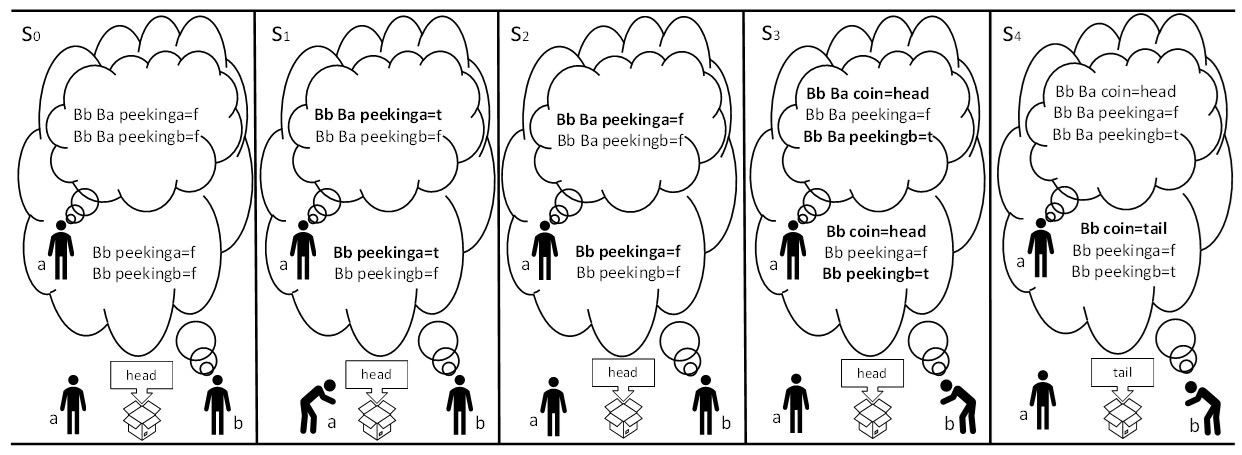
\includegraphics[width=0.9\textwidth]{Figures/plan_2_final.jpg}
    \caption{Plan~\ref{plan2} with agent $b$'s justified beliefs. Bold text indicates the belief that has changed.}
    \label{fig:plan_2_final}
\end{figure*}

\begin{example}
\label{example:coin}
There are two agents, $a$ and $b$, and there is a coin $c \in \{head,\ tail\}$ inside a box. 
The coin can only be seen by the agents when they are peeking into the box.
The agents can see each other all the time, which means they see whether others are peeking into the box. 
The actions that agents can take are ``\emph{peek}'' and ``\emph{return}'', while the coin can ``\emph{flip}'' itself at any point in time. The action and outcome of the flip is only visible to the agents who are peeking into the box.
Initially, both agent $a$ and $b$ are not peeking, and the coin is $head$.
The task is to generate a false belief such that: 
\begin{enumerate}
    \item the coin is $tail$;
    \item agent $b$ believes that the coin is $tail$; 
    \item agent $a$ believes that the coin is $head$; and 
    \item agent $b$ believes that agent $a$ believes that the coin is $head$.
\end{enumerate}
% 1. the coin is $tail$; 
% 2. agent $b$ believes the coin is $tail$; 
% 3. agent $a$ believes the coin is $head$; and 
% 4. agent $b$ believes that agent $a$ believes the coin is $head$.

\end{example}

% \begin{figure*}[h]
%     \centering
%     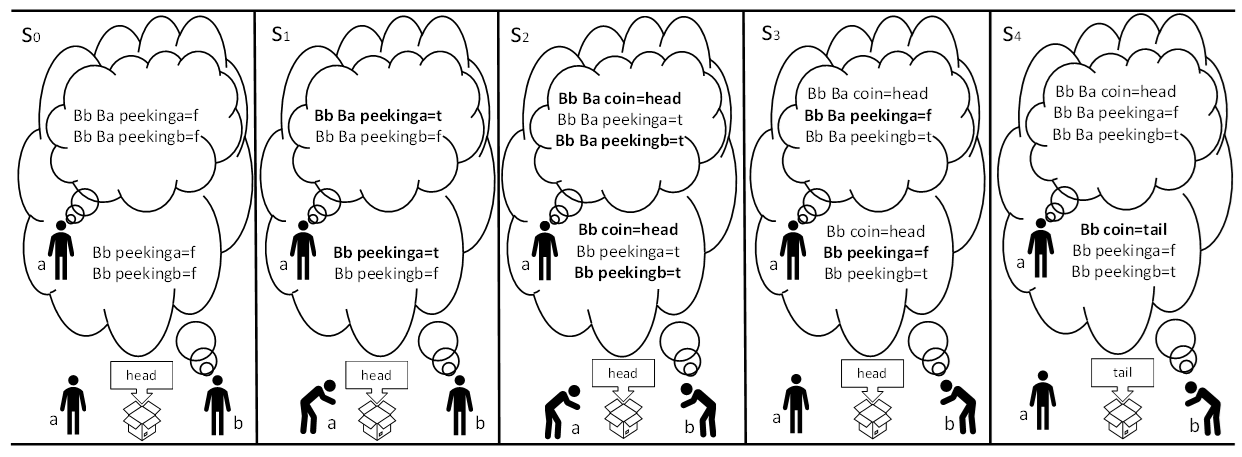
\includegraphics[width=0.9\textwidth]{Figures/plan_1_final.png}
%     \caption{Plan~\ref{plan1} with agent $b$'s justified beliefs. Bold text indicates belief that has changed.}
%     \label{fig:plan_1_final}
% \end{figure*}


% \begin{figure}
%     \centering
%     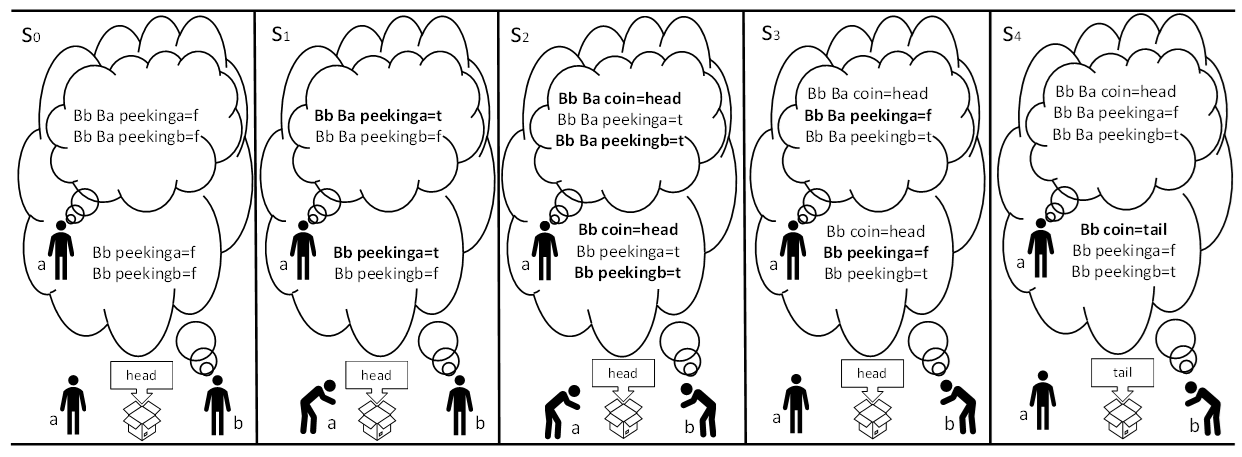
\includegraphics[width=0.95\columnwidth]{Figures/plan_1_final.png}
%     \caption{ Plan~\ref{plan1} to solve Example~\ref{example:coin}}
%     \label{fig:coin_plan_A}
% \end{figure}

% \tm{If you need to save space, I suggest dropping Plan 1.1 and just having Plan 1.2, which illustrates both of the main issues. If you have the space, keep both because the incremental building from 1.1 to 1.2 is nice}
% \gh{I am keeping a simplified version of plan 1.1}

A valid plan would be:
\begin{plan}
\label{plan1}
\emph{peek(a)}, \emph{peek(b)}, \emph{return(a)}, \emph{flip}
\end{plan}
It is intuitive that $B_b B_a coin=head$ holds, because agent $b$ saw agent $a$ peeked into the box after the action $\emph{peek(b)}$ and agent $a$ was not peeking into the box while $coin$ flipped.


\begin{comment}
A valid plan would be:
\begin{plan}
\label{plan1}
\emph{peek(a)}, \emph{peek(b)}, \emph{return(a)}, \emph{flip}
\end{plan}


As shown in Figure~\ref{fig:plan_1_final}, each criteria is reasoned as follows: 
\begin{enumerate}
    \item the coin becomes $tail$ in $s_4$; 
    \item agent $b$ believes (actually knows!) the coin is $tail$ as $b$ is peeking into the box in $s_4$; 
    \item agent $a$ believes coin is $head$ because the last state $a$ peeked into box is $s_2$ and the coin was $head$ in $s_2$, and has no evidence to disregard this;
    \item agent $b$ believes agent $a$ believes coin is $head$ because the last state $b$ saw $a$ peeking into the box is $s_2$ and the coin was $head$ in $s_2$. 
\end{enumerate}

Item 2 and 4 are worth discussing. 
For item 2, in state $s_4$, agent $a$ does not observe what is inside the box (the value of the coin).
Agent $a$ rather recalls the last time it saw the value of the $coin$ is $s_2$, and $a$ should ``remember'' the $coin$ is $head$.
For item 4, in  state $s_4$, agent $b$ observes that agent $a$ is not peeking into the box.
So, agent $b$ recalls that the last time $b$ saw $a$ see the value of the $coin$ was $s_2$ ($S_a coin$). 
Although it might be intuitive to use the value of the $coin$ from state $s_2$ to form the justified believe $B_b\ B_a coin=head$, the value we use should come from what agent $b$ believes the value was when agent $a$ peeked. 
It might look equivalent when analysing Plan~\ref{plan1}, but the former may lead the agent to hold no belief or a false-belief of the value compared to the actual value.
\end{comment}
% 1. the coin becomes $tail$ in $s_4$; 
% 2. agent $b$ believes (actually knows!) coin is $tail$ as $b$ is peeking into the box in $s_4$; 
% 3. agent $a$ believes coin is $head$ because the last state $a$ peeked into box is $s_2$ and coin was $head$ in $s_2$;
% 4. agent $b$ believes agent $a$ believes coin is $head$ because the last state $b$ saw $a$ peeking into the box is $s_2$ and the coin was $head$ in $s_2$. 

% \begin{figure}
%     \centering
%     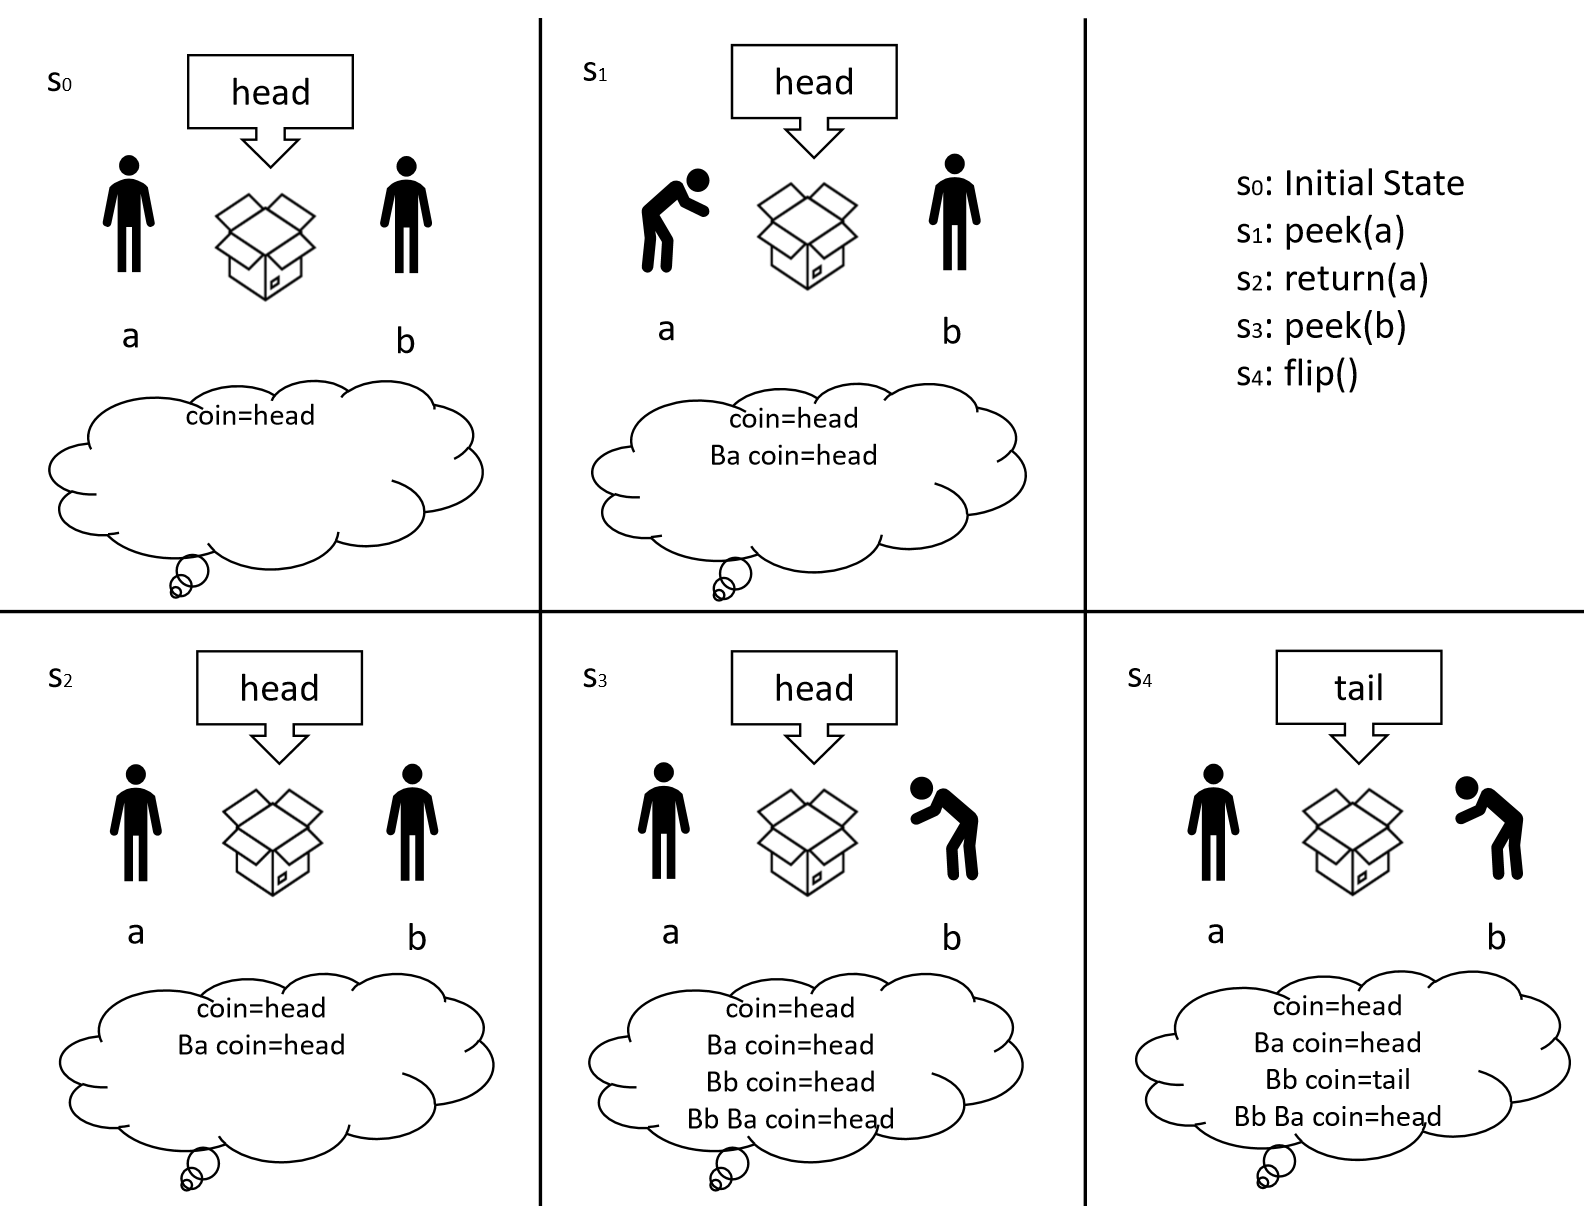
\includegraphics[width=0.9\columnwidth]{Figures/coin_plan2.png}
%     \caption{ Plan~\ref{plan2} to solve Example~\ref{example:coin}}
%     \label{fig:coin_plan_B}
% \end{figure}

A more challenging  plan to reason about, shown in Figure~\ref{fig:plan_2_final}), is:
\begin{plan}
\label{plan2}
\emph{peek(a)}, \emph{return(a)}, \emph{peek(b)}, \emph{flip}
\end{plan}



In this plan, agent $a$ and $b$ no longer peek into the box at the same time, which means, we do not have $K_b K_a coin=head$ in state $s_2$.
All criteria are met as in Plan~\ref{plan1}, except item 4.
For item 4, similarly, agent $b$ recalls that the last time it saw agent $a$ seeing the coin ($S_a coin$) was $s_1$.
However, agent $b$ holds no knowledge or belief on the value of the $coin$ from $s_1$, which means she cannot generate the justified belief in $s_1$.
Fortunately, agent $b$ gains belief of the coin from $s_3$.
So, agent $b$ still can justify its belief $B_b\ B_a coin=head$:
\begin{enumerate}
    \item $b$ recalls that the last time agent $a$ peeked inside of the box is $s_1$; and
    \item after $b$ saw $a$ peek, the next time $b$ saw the value of the $coin=head$ is at state $s_3$.
\end{enumerate}

In a model-free setting, reasoning about this is particularly challenging. 
Agents do not have access to the action model, so they cannot reason about what other agents have seen. 
Instead, they can only partially observe states and re-construct belief by observing states and who else observes each state.

This paper presents a model for KD45$_n$ belief over such plans, with the ability to solve model-free problems. Instead of keeping track of all possible beliefs, we instead use a lazy-evaluation approach that searches through previous states of the plan to re-construct what has been seen, and by who, to evaluate nested belief formulae. Our results show that we can efficiently solve existing benchmarks in epistemic and doxastic planning, even with a simple prototype planner.


% As shown in the Figure~\ref{fig:coin_plan_B}: 
% 1. the coin becomes $tail$ in $s_4$; 
% 2. agent $b$ believes (actually knows!) coin is $tail$ as $b$ is peeking into the box in $s_4$; 
% 3. agent $a$ believes coin is $head$ because the last state $a$ peeked into box is $s_2$ and coin was $head$ in $s_2$;
% 4. agent $b$ believes agent $a$ believes coin is $head$ because the last state $b$ saw $a$  peeking into the box is $s_2$ and the coin was $head$ in $s_2$. 



% The ability to reason about ones knowledge or belief beyond observation is another intelligent behaviour for epistemic agents. 
% Considering the following BBL example, which agents must be reason about two variables that they cannot observe at the same time.

% \tm{It is not clear to me that this BBL example gives much of a better idea than the coin task}

% \begin{example}
% \label{example:bbl}
% Agent $a$ and $b$ are two stationary cameras with certain vision range ($90^\circ$), and there is a target $x \in \{armed,\ unarmed\}$.
% Agent $b$ and target $x$ are located on the each side of agent $a$, which indicates that agent $a$ cannot see them both at the same moment.
% Agents do not know the location of each other nor target unless its within their sight. 
% The actions that agents can take is ``\emph{turn}'' and targets can take are ``\emph{pickup}'' and ``\emph{drop}''.
% Initially, agent $a$ faces west ($180^\circ$), agent $b$ faces west ($180^\circ$) and target $x$ is $armed$.
% The task is to generate a belief such that:
% 1. the target $x$ is $armed$;
% 2. agent $b$ knows the target $x$ is $armed$;
% 3. agent $a$ believes that agent $b$ knows the target $x$ is $armed$
% \end{example}
% % The two variables lies in separate boxes, and each agent is only able to look into one of the box at a time. In addition, agents know which box each other are looking at the moment.  

% % Example 1.0: Initially, let $x,y=1$ and $i \triangleright b_x, j \triangleright b_x$. Then, let us assume that agent $j$ looks away (e.g. turn to peek $b_y$), and the agent $i$ change the value of $x$ in box $b_x$ into $2$.
% To allow agent $a$ reason about agent $b$'s knowledge, agent $a$ needs to turn to be able to see agent $b$, $turn(-180^\circ)$, etc..
% Then, following the PWP model, agent $a$'s perspective contains agent $a$ and agent $b$ (target $x$ is not there).
% That is, agent $a$ can only reason about $b$'s perspective from $a$'s perspective of the world.
% Clearly, (3) does not hold as target $x$ is not in agent $a$'s perspective at all.
% It is obvious that some useful information, such as agent $a$ in the past knows target $x$ is $armed$, has lost during this process.

% Example 2.0: Can an agent gain the belief such as $x+y=2$?

% The tricky part is in this domain, agent is never able to see both variables at the same moment. So, that agent's belief about $x+y$ could be generated based on its belief over $x$ and $y$ separately rather than the belief over the relation $x+y$ as a whole.


